\section{Checkpoint/Restore of Established Connections} \label{sec:system}

The ability to checkpoint established TCP connection is mainly due to the inclusion of the \texttt{TCP\_REPAIR} socket option to kernel version $3.5$~\cite{tcp-connection-repair}.

\subsection{Implementation in \criu}

Similarly to other resources and as introduced in \S\ref{sec:background}, basic information about sockets is obtained by parsing the adequate files in the \texttt{/proc} filesystem.
However, there are some internals of active network connections (namely negotiatied parameters such as send and receive queues, and sequence numbers) that require putting the socket in the \texttt{TCP\_REPAIR} state using the \texttt{setocketopt()} syscall (note that this action requires \texttt{CAP\_NET\_ADMIN} capabilities).
Then, if the connection is closed whilst the socket is in \texttt{TCP\_REPAIR} mode, no \texttt{FIN} nor \texttt{RST} packets are sent to the other peer, what means that his endpoint is effectively still open~\cite{Corbet12}.

To re-establish the connection from the newly generated socket, the first thing to do is put it, again, in \texttt{TCP\_REPAIR} mode.
Then, the previously dumped parameters can be set, and upon \texttt{connect()} the socket goes directly into \texttt{ESTABLISHED} mode without acknowledgment from the other end, and a \texttt{RST} packet is sent to resume communication.

% TABLE FILTERING
The last missing piece is what happens is the remote end tries to send a packet to its, seemingly open, TCP socket whilst the other peer is down.
Were we to ignore this fact, once the packet reached our kernel this, given that the socket is closed, would send a \texttt{RST} to the other end, and our whole illusion would collapse.
To overcome this issue, upon checkpoint we include a set of rules to the \texttt{netfilter}~\cite{netfilter} IP routing table to drop all packets.
We include the set of rules in Table~\ref{table:iptables-rules}.
\begin{table}[h!]
    \centering
    {\ttfamily 
    \begin{tabular}{p{1.2cm}p{0.5cm}p{0.5cm}p{0.7cm}p{0.7cm}p{2.0cm}}
        \multicolumn{6}{l}{Chain INPUT (policy ACCEPT)} \\
        target & prot & opt & source & dest & \\
        CRIU & all & -- & .../0 & .../0 & \\
        & & & & & \\
        \multicolumn{6}{l}{Chain FORWARD (policy ACCEPT)} \\
        target & prot & opt & source & dest & \\
        & & & & & \\
        \multicolumn{6}{l}{Chain OUTPUT (policy ACCEPT)} \\
        target & prot & opt & source & dest & \\
        CRIU & all & -- & .../0 & .../0 & \\
        & & & & & \\
        \multicolumn{6}{l}{Chain CRIU} \\
        target & prot & opt & source & dest & \\
        ACCEPT & all & -- & .../0 & .../0 & mark 0xc114 \\
        DROP & all & -- & .../0 & .../0 & \\
    \end{tabular}
    }
    \caption{Output of running \texttt{iptables -t filter -L -n}.\label{table:iptables-rules}}.
\end{table}

\subsection{How to efficiently reuse IP addresses?}

A caveat of restoring established TCP connections is that, without bringing down both peers, we can not circumvent the negotiated \texttt{IP:PORT} pairs.
As a consequence, the same IP address and port must be available at restore time, otherwise when the remote peer receives the \texttt{RST} package it will immediately close the connection.
Re-using an IP address is achievable using locally scoped addresses or network namespaces.
In our experiments we tested both.

Firstly, if we are migrating into a different machine (as the experiments presented in \S\ref{sec:evaluation}), we need to assign addresses using \texttt{ip}'s \texttt{addr} subcommands.
In particular, we are using a \texttt{host-only}~\cite{vbox-hostonly} subnet to manage our (virtual) machines.

Alternatively, we have also tested process migration within the same machine, from one network namespace to a different one.
This situation is particularly interesting as it recreates what happens under the hood in \criu's binding for \runc, as containers rely on namespaces for isolation.
We set up a bridge device in the host namespace, two network namespaces, and two virtual ethernet devices with one peer tied to the bridge, and the other one inside a namespace.
Adequately setting up addresses and default gateway routes, we achieve the setup we depict in Figure~\ref{fig:veth-arch}.
\begin{figure}[h!]
    \centering    
    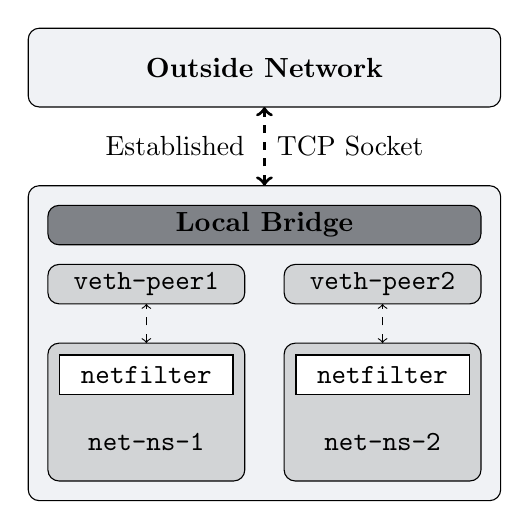
\begin{tikzpicture}
        % Color definition
        \definecolor{machineBG}{RGB}{240, 242, 245}
        \definecolor{namespaceBG}{RGB}{210, 212, 214}
        \definecolor{bridgeBG}{RGB}{127, 130, 135}

        % Host network box
        \draw[fill=machineBG, rounded corners] (0,0) rectangle (6, 4);
        % Network Namespace 1 and Peer
        \draw[fill=namespaceBG, rounded corners] (0.25, 0.25) rectangle (2.75, 2.0);
        \node at (1.5, 0.75) {\textbf{\texttt{net-ns-1}}};
        \draw[fill=white] (0.4, 1.35) rectangle (2.6, 1.85) node[pos=.5] {\text{\texttt{netfilter}}};
        \draw[<->, dashed] (1.5,2) -- (1.5,2.5);
        \draw[fill=namespaceBG, rounded corners] (0.25, 2.5) rectangle (2.75, 3) node[pos=.5] {\text{\texttt{veth-peer1}}};
        % Network Namespace 2
        \draw[fill=namespaceBG, rounded corners] (3.25, 0.25) rectangle (5.75, 2.0);
        \node at (4.5, 0.75) {\textbf{\texttt{net-ns-2}}};
        \draw[fill=white] (3.4, 1.35) rectangle (5.6, 1.85) node[pos=.5] {\text{\texttt{netfilter}}};
        \draw[<->, dashed] (4.5,2) -- (4.5,2.5);
        \draw[fill=namespaceBG, rounded corners] (3.25, 2.5) rectangle (5.75, 3) node[pos=.5] {\text{\texttt{veth-peer2}}};
        % Local Bridge
        \draw[fill=bridgeBG, rounded corners] (0.25, 3.25) rectangle (5.75, 3.75) node[pos=.5] {\textbf{Local Bridge}};

        % Connecting line
        \draw[<->, dashed, very thick] (3,4) -- (3,5) node[pos=.5] {Established \hspace{5pt} TCP Socket};

        % Outside network box
        \draw[fill=machineBG, rounded corners] (0,5) rectangle (6, 6) node[pos=.5] {\textbf{Outside Network}};
    \end{tikzpicture}
    \caption{Architecture of three different namespaces connected through virtual ethernet pairs.\label{fig:veth-arch}}
\end{figure}

\subsection{Live migration and integration with \runc}

Integration with \runc is two-fold.
For the TCP connection \criu's binding for \runc includes a \texttt{--tcp-established} flag that does most of the socket management.
If we are interested in restoring the connection in a different machine or namespace, we must manually recreate the filter table from Table~\ref{table:iptables-rules} using the \texttt{iptables} command.
Lastly, to restore into an existing namespace, the container must be restored with the adequate open file descriptors using \criu's \texttt{--external}~\cite{criu-external} and \texttt{--inherit-fd}~\cite{criu-inherit-fd}.
